\documentclass{standalone}
\usepackage{tikz}

\begin{document}

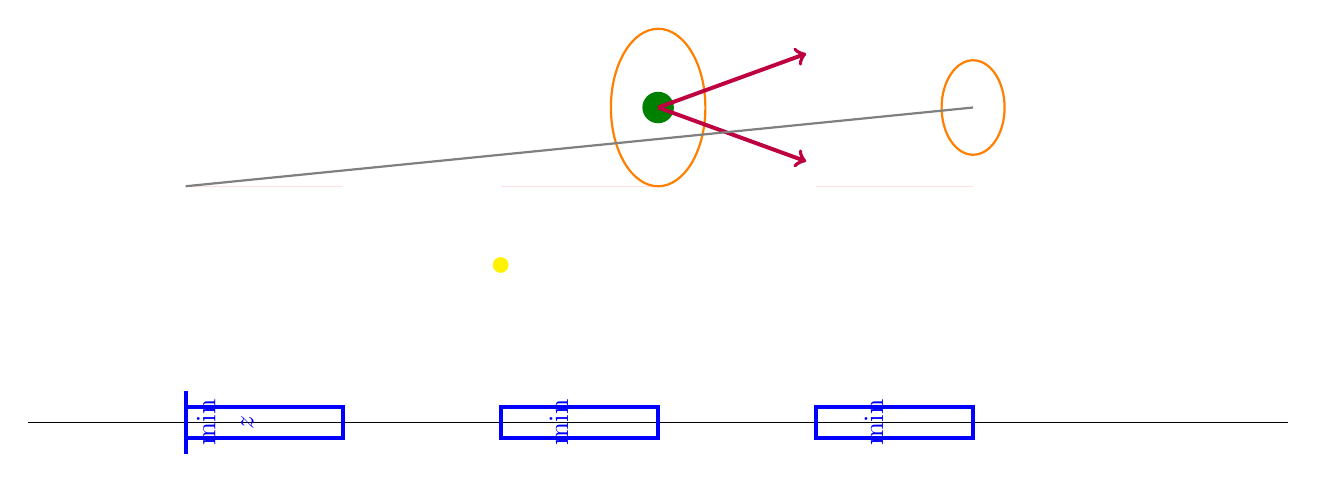
\begin{tikzpicture}[scale=2]

% Draw the horizontal lines representing the ground
\draw (-4,0) -- (4,0);

% Define the buildings and their heights
\def\buildingheight{1.5}
\def\minheight{0.8}

% Draw the first building
\fill[red] (-3,\buildingheight) rectangle ++(1,0);
\draw[blue, line width=0.5mm] (-3,-0.1) rectangle ++(1,0.2) node [midway, above, rotate=90] {\textcolor{blue}{$z$}};
\draw[blue, line width=0.5mm] (-3,-0.2) -- ++(0,0.4) node [midway, below, rotate=90] {\textcolor{blue}{$\min$}};

% Draw the second building
\fill[red] (-1,\buildingheight) rectangle ++(1,0);
\draw[blue, line width=0.5mm] (-1,-0.1) rectangle ++(1,0.2) node [midway, above, rotate=90] {\textcolor{blue}{$\min$}};

% Draw the third building
\fill[red] (1,\buildingheight) rectangle ++(1,0);
\draw[blue, line width=0.5mm] (1,-0.1) rectangle ++(1,0.2) node [midway, above, rotate=90] {\textcolor{blue}{$\min$}};

% Draw the transmitter and receiver positions
\fill[green!50!black] (0,\buildingheight+0.5) circle (0.1) node [above] {};
\fill[yellow] (-1,\buildingheight-0.5) circle (0.05) node [below, yshift=-1ex] {};

% Draw the antenna pattern
\draw[orange, thick] (0,\buildingheight+0.5) ellipse (0.3 and 0.5);
\draw[orange, thick] (2,\buildingheight+0.5) ellipse (0.2 and 0.3);

% Draw the elevation angles
\draw[purple, line width=0.5mm, ->] (0,\buildingheight+0.5) -- ++(20:1);
\draw[purple, line width=0.5mm, ->] (0,\buildingheight+0.5) -- ++(-20:1);

% Draw the line of sight (LoS) path
\draw[gray, thick] (-3,\buildingheight) -- (2,\buildingheight+0.5);

\end{tikzpicture}

\end{document}